\chapter{文献综述与理论基础}
\label{chap:lit}

本章分两部分。前一部分按六条线索梳理与研究问题直接相关的文献：再生数的定义与估计、超传播与过度离散、漏报与报告过程、估计精度的信息论刻画、环境随机性、监测设计与预测评价。每条线索都说明它为第三章的模型提供了哪个组成部分，以及它在估计目标问题上留下了什么没有回答。后一部分整理第三、四章要用到的概率与统计工具，包括分支过程与概率生成函数、负二项分布的混合表示与抽稀性质、全方差公式、信息不等式与一致最小方差无偏估计、单调似然比检验，以及两阶段抽样的方差结构。

\section{再生数的定义与估计方法}
\label{sec:lit-rt}

\subsection{基本再生数与时变再生数}

基本再生数 $R_0$ 刻画完全易感人群中一名典型感染者产生的继发感染数，是传染病动力学的核心参数\citep{anderson1991infectious, keeling2008modeling}。在异质人群中，$R_0$ 被定义为下一代算子的主特征值\citep{diekmann1990definition}，这一定义把不同类型个体之间的传播矩阵压缩为一个阈值量。流行开始后，易感者比例下降、干预措施实施、接触模式变化，传播强度随时间改变，时变再生数 $R_t$ 用于描述第 $t$ 期的实际传播水平。

再生数与可观测的增长率之间的换算依赖世代间隔分布。Wallinga 与 Lipsitch 指出，由增长率推断再生数的多种公式只在假定的世代间隔分布形状上不同，世代间隔分布的形状决定了应采用哪一个换算式\citep{wallinga2007generation}。对流感而言，家庭传播研究估计的序列间隔均值为数天：一项家庭随访研究估计为 3.6 天\citep{cowling2009estimation}，一项系统综述对季节性 H3N2 流感与 2009 年大流行流感分别估计为 2.2 天和 2.8 天\citep{vink2014serial}。这些估计都短于一周，因此在按周汇总的流感数据中，一周大致对应一代多一点的传播，按代建立的模型可以近似套用到周数据上，第五章使用的滞后权重即依此设定。

\subsection{基于更新方程的估计}

实时估计 $R_t$ 的主流方法建立在更新方程上。Wallinga 与 Teunis 用世代间隔分布把每个病例归因到可能的感染源，得到逐病例的再生数\citep{wallinga2004different}；Fraser 把更新方程写成发病数关于此前发病数的卷积，给出实时估计的框架\citep{fraser2007estimating}。Cori 等在滑动窗口内假定 $R_t$ 不变，并假设病例计数服从泊松分布，用 Gamma 共轭先验得到 $R_t$ 后验的闭式表达\citep{cori2013new}，这一方法因实现简单而被广泛使用。Thompson 等在此基础上把序列间隔的不确定性纳入估计，并区分本地病例与输入病例\citep{thompson2019improved}。Nouvellet 等给出同一框架下的简单发病预测方法\citep{nouvellet2018simple}。

方法使用中的实际问题也已有系统讨论。Gostic 等比较了多种估计方法，指出报告延迟、右删失和窗口选择会使实时估计产生偏差，并给出相应的修正建议\citep{gostic2020practical}。Abbott 等用病例与死亡数据在滚动窗口内估计全球到地方各级的时变再生数，显式处理报告延迟的不确定性，使估计基于潜在感染而非报告数\citep{abbott2020estimating}。Bettencourt 与 Ribeiro 以可观测量构建病例数的概率递推模型，对有效再生数做实时贝叶斯估计，并据此构造检验以识别异常\citep{bettencourt2008real}。窗口长度的选择也被单独研究：Parag 与 Donnelly 把 $R_t$ 写成分段常数函数，用最小描述长度原则选择分段数，避免分段过少导致的欠拟合与分段过多导致的过拟合\citep{parag2020adaptive}。半机制贝叶斯模型把更新方程、报告过程和潜在感染统一在一个层次模型中\citep{bhatt2023semi}，序贯蒙特卡洛方法则为这类模型提供了在线推断工具\citep{steyn2025primer}。大流行期间，这些框架被用于估计非药物干预的效果\citep{flaxman2020estimating}和早期传播动力学\citep{kucharski2020early}。

上述文献关注的是如何在给定数据上得到偏差小、不确定性刻画准确的 $R_t$ 估计。估计目标默认是当期 $R_t$，后验或置信区间的宽度随病例数增加而收窄。至于决策者关心跨期平均水平时误差如何随规模变化，这些文献没有单独讨论。

\section{超传播与负二项后代分布}
\label{sec:lit-superspreading}

\subsection{个体传染力的异质性}

同一种疾病的感染者之间传染力差异很大。Lloyd-Smith 等把个体再生数 $\nu$ 设为均值为 $R$、形状参数为 $k$ 的 Gamma 分布，继发感染数在给定 $\nu$ 时服从泊松分布，由此得到负二项后代分布，并在多种疾病的暴发数据上估计 $k$\citep{lloydsmith2005superspreading}。$k$ 越小，个体差异越大，少数人造成大部分传播的现象越明显。Galvani 与 May 的评论指出，个体传染性差异使超传播疾病容易引发爆发式流行，同样的波动也使暴发更容易自行熄灭\citep{galvani2005dimensions}。

在新发传染病中，离散参数 $k$ 的估计受到重视。Blumberg 与 Lloyd-Smith 用传播链规模分布同时估计 $R_0$ 与 $k$，指出 $R_0$ 的点估计只取决于平均链长，其置信区间却依赖于推断出的异质性程度\citep{blumberg2013inference}。Endo 等用中国以外地区的暴发规模估计 2019 冠状病毒病的过度离散参数，结论支持高度的传播异质性\citep{endo2020estimating}。Adam 等基于中国香港 1038 例病例的接触追踪数据估计，19\% 的病例造成了 80\% 的本地传播\citep{adam2020clustering}。

\subsection{负二项后代分布的形状}

图~\ref{fig:offspring} 用示例参数 $R=1.15$ 展示离散参数对后代分布的影响。左图为继发感染数的概率分布，纵轴取对数。$k=0.35$ 时一名感染者不产生任何继发感染的概率为 0.6009，$k=0.1$ 时升至 0.7768，同等均值下的泊松分布只有 0.3166。离散程度越高，零后代的概率越大。与泊松分布相比，负二项分布的右尾也厚得多：在 8 个继发感染处，$k=0.1$ 与 $k=0.35$ 的概率分别是泊松分布的 267 倍和 299 倍。$k=0.1$ 把更多概率放在零和更远的尾部，所以在 8 处略低于 $k=0.35$。均值相同而形状差异如此之大，说明只看平均传播强度会掩盖传播过程的随机性。

右图为传播集中度曲线。横轴是按个体再生数从高到低排序后的感染者比例，纵轴是这部分感染者贡献的期望传播份额，计算时利用了 Gamma 分布的尺寸偏倚性质，份额与 $R$ 无关。传染力最强的 20\% 感染者，在 $k=0.1$、0.35、1 时分别贡献 95.1\%、72.4\% 和 52.2\% 的传播；若所有人传染力相同，这一比例为 20\%，对应图中的对角虚线。$k=0.35$ 位于常见呼吸道传染病估计值的范围内\citep{lloydsmith2005superspreading}，这时七成以上的传播集中在两成的人身上。

\begin{figure}[!tbp]
  \centering
  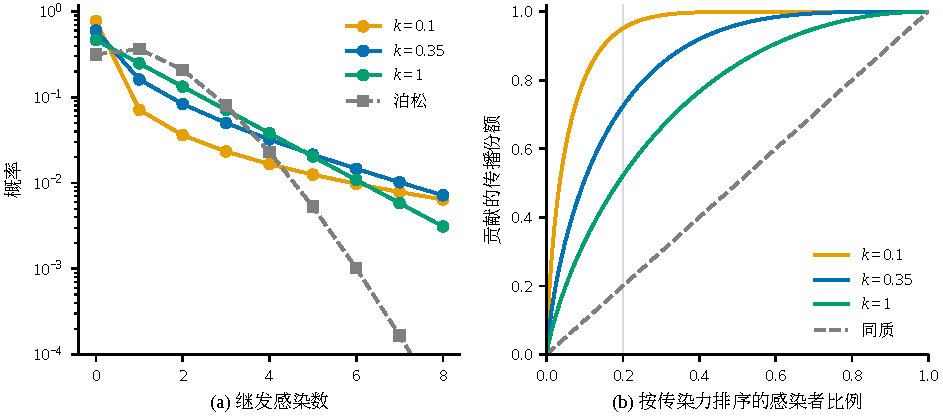
\includegraphics[width=\textwidth]{figures/fig_2_1_offspring.pdf}
  \caption{负二项后代分布与传播集中度。（a）均值 $R=1.15$ 时不同离散参数下继发感染数的概率分布，纵轴为对数刻度，虚线为同均值的泊松分布。（b）按个体再生数排序后，前一定比例感染者贡献的期望传播份额，竖线标出 20\% 处。}
  \label{fig:offspring}
\end{figure}

这种集中性对监测统计量有直接影响。一期报告病例的方差除了泊松部分 $R$ 外，还多出 $R^2/k$ 一项，第三章将看到这一项在报告完整时依然存在，只有扩大观测的感染者人数才能把它平均掉。超传播文献主要讨论 $k$ 对疫情暴发概率和防控策略的影响，较少把 $k$ 放进监测统计量的方差分解。

\subsection{分支过程理论}

负二项后代分布可以嵌入 Galton--Watson 分支过程。Harris 的专著系统建立了分支过程理论，覆盖 Galton--Watson 过程、Markov 分支过程和年龄依赖过程\citep{harris1963theory}；Athreya 与 Ney 对分支过程的极限理论作了统一处理\citep{athreya1972branching}。在流行早期，易感者耗竭可以忽略，感染者之间相互独立地产生后代，分支过程是传播的自然近似。第三章的单代模型正是一个带环境的分支过程中相邻两代之间的一步转移。

\section{漏报与报告过程}
\label{sec:lit-reporting}

\subsection{漏报的层级与规模}

监测系统记录的病例只是全部感染的一部分。Gibbons 等把漏报分为两个层级：社区中的感染者未就医，以及就医后未被报告；文献中的乘数因子在疾病和国家之间差异很大\citep{gibbons2014measuring}。Reed 等对 2009 年美国甲型 H1N1 流感的估计表明，截至当年 7 月实验室确诊的报告病例约 4.4 万例，校正漏检后实际感染估计为 180 万至 570 万例\citep{reed2009estimates}。对于住院监测，报告率可以理解为感染者中住院并被记录的比例。季节性流感的有症状侵袭率\citep{tokars2018seasonal}与住院负担\citep{zhou2012hospitalizations, rolfes2018annual}共同决定了这一比例的量级，第三章的住院情景取 0.0056 至 0.021 即由此得到。美国每个流感季的流感相关住院估计为 14 万至 71 万例\citep{rolfes2018annual}，州级周报的住院数因此在数个到数千个之间变化，为第五章检验规模效应提供了足够宽的规模范围\citep{cdc2026nhsn}。

\subsection{漏报的建模方法}

漏报对再生数估计的影响有两类处理方法。一类在估计中直接修正报告偏差：Azmon 等研究了误报数据下的再生数估计\citep{azmon2014estimating}；Stoner 等提出分层模型修正计数数据中的漏报\citep{stoner2019hierarchical}；Bracher 与 Held 用边际矩匹配方法拟合漏报数据下的地方性与流行性模型\citep{bracher2021marginal}。另一类把报告过程写成对真实计数的随机抽稀。Steutel 与 van Harn 引入的二项抽稀算子用伯努利随机变量之和代替常数乘法，保持取值为非负整数\citep{steutel1979discrete}；Al-Osh 与 Alzaid 基于这一算子提出一阶整数值自回归模型，其相关结构类似连续的一阶自回归\citep{alosh1987first}。计数回归的系统处理可见 Cameron 与 Trivedi 的专著\citep{cameron2013regression}。

二项抽稀的好处在于它与负二项分布相容：负二项变量经二项抽稀后仍服从负二项分布（见第~\ref{sec:lit-tools} 节）。这使报告病例数的条件分布有显式形式，估计量的精确性质可以写出来。报告完整与否在这种表示下只改变一个参数，报告率与覆盖面两条扩容途径的效果因而可以在同一个式子里比较。

漏报还带来测量误差问题。若用于归一化的病例规模本身含噪，回归系数会偏离真实值，这是测量误差文献中的经典结论\citep{fuller1987measurement, carroll2006measurement}。第五章解释经验斜率偏大时会用到这一点。

\section{估计精度的信息论刻画}
\label{sec:lit-information}

Fisher 信息与 Cramér--Rao 不等式是刻画估计精度上限的标准工具。Rao 给出了无偏估计量方差不低于 Fisher 信息倒数的下界\citep{rao1945information}，Cramér 在其专著中独立得到同一结果\citep{cramer1946mathematical}；现代教材把它与指数族、充分统计量和完备性联系起来\citep{casella2002statistical, lehmann1998point}。若一个无偏估计量的方差恰好等于这一下界，它在无偏估计量中是最有效的。

Parag 等把这一工具引入传染病监测。在泊松更新模型下，再生数的 Fisher 信息与窗口内的总感染压力成正比，病例越多，信息越多，估计越精确\citep{parag2022quantifying}。Parag 与 Donnelly 进一步讨论了实时推断疫情反弹的基本极限\citep{parag2022fundamental}，Parag 等又分析了带噪数据对及时干预的非对称限制：判断疫情在增长和判断疫情在下降所需的时间并不相同\citep{parag2025asymmetric}。这些结果针对的都是当期再生数，信息随病例数线性增长，与第三章的目标Ⅰ一致。

信息论方向的研究留下两处可以延伸的地方。一处是过度离散，泊松假设下信息随病例数线性增长，负二项假设下信息的表达式会多出一个与 $k$ 有关的项，需要重新推导。另一处是估计目标，若关心的量是跨期平均水平，当期 $R_t$ 围绕平均水平的波动是一项额外的误差，它不进入当期 $R_t$ 的 Fisher 信息，却决定了平均水平估计的精度上限。

\section{环境随机性}
\label{sec:lit-environment}

\subsection{生态学中的两类随机性}

种群生态学长期区分两类随机性。人口随机性来自个体出生、死亡等事件的独立随机性，环境随机性来自所有个体共同承受的外部波动。Engen 等给出了两者的严格定义：人口随机性对种群增长率方差的贡献与种群规模成反比，环境随机性的贡献不随规模变化\citep{engen1998demographic}。Lande 等的专著把这一区分作为随机种群动力学的出发点\citep{lande2003stochastic}，Bj{\o}rnstad 与 Grenfell 的综述讨论了确定性动力学、密度依赖与随机强迫的相互作用\citep{bjornstad2001noisy}。大种群中人口随机性被平均掉，种群波动主要由环境随机性驱动。

\subsection{传染病中的环境随机性}

传染病动力学同样受两类随机性共同驱动。Rohani 等分析了儿童传染病中确定性与随机性的相互作用\citep{rohani2002determinism}。Bret\'o 等提出基于机制模型的时间序列分析方法，在传播率中加入环境噪声\citep{breto2009time}；He 等用仅需模型模拟的推断方法分析麻疹数据，指出纳入超出人口随机性的额外噪声对处理环境随机性和模型误设很重要\citep{he2010plug}。Rasmussen 等结合基因谱系与时间序列推断随机环境下的传播参数\citep{rasmussen2011inference}。

流感传播的环境驱动因素已有较多实证证据。Shaman 与 Kohn 重新分析实验数据，发现绝对湿度解释了 50\% 的流感病毒传播变异和 90\% 的病毒存活变异\citep{shaman2009absolute}；Shaman 等进一步发现美国流感季的起始与此前数周绝对湿度异常偏低相关，用观测湿度调节传播率即可复现流感的季节周期\citep{shaman2010absolute}。Dalziel 等表明城市化程度与湿度共同塑造美国城市流感流行的强度\citep{dalziel2018urbanization}。这些研究说明，同一辖区同一时期的感染者共享随时间变化的环境，各期 $R_t$ 围绕平均水平的波动有实在的物理与社会来源。

生态学的两类随机性区分尚未被系统地用于监测统计量的精度分析。环境波动在生态学中决定种群灭绝风险，在监测问题中则决定跨期平均水平估计的精度底板。把两者对应起来，需要在监测数据的生成机制中显式写出环境层，并说明观测规模与人口随机性部分的关系。

\section{监测设计与抽样理论}
\label{sec:lit-design}

\subsection{监测系统的设计与评价}

监测系统的设计长期依赖经验规则和定性评价。美国疾病控制与预防中心发布的监测系统评价指南从有用性、简单性、灵活性、数据质量、灵敏度、代表性和及时性等方面评价监测系统\citep{german2001updated}，但没有给出规模与精度之间的定量关系。哨点选址研究给出了一些定量证据：Polgreen 等用最大覆盖模型为美国爱荷华州的流感哨点选址，发现新增站点的人口覆盖呈边际收益递减，10 个优化站点即可达到现有 22 个站点的覆盖率\citep{polgreen2009optimizing}。Scarpino 等利用历史监测数据优化得克萨斯州的哨点招募，优化后的网络用较少的哨点就能优于现有网络，原因在于避免了信息冗余\citep{scarpino2012optimizing}。

这些研究的优化目标是人口覆盖率或与参考序列的拟合程度，收益递减来自站点之间的信息重叠。规模收益递减还有一个来源，即环境项不随规模下降，监测设计文献很少从估计方差的结构推出环境底板。

\subsection{两阶段抽样与方差分量}

抽样调查理论为讨论规模收益提供了现成框架。两阶段抽样先抽初级单元，再在每个初级单元内抽次级单元，估计量的方差由初级单元间方差和初级单元内方差两部分组成，前者只能通过增加初级单元数来降低\citep{cochran1977sampling}。Cochran 给出了在线性费用函数下初级单元内最优样本量的公式，Kish 提出的设计效应把整群抽样的方差膨胀归结为组内相关\citep{kish1965survey}，Lohr 的现代教材对这些结果作了系统整理\citep{lohr2022sampling}。方差分量的估计方法可见 Searle 等的专著\citep{searle1992variance}。

监测问题与两阶段抽样在结构上相似。各观测期可以看作初级单元，环境方差对应初级单元间方差，人口随机性与报告过程对应初级单元内方差。两者的差别在于独立性：抽样调查中初级单元按设计独立抽取，监测数据中的各期环境可能存在时间相关，次级单元的数目也由此前的传播产生。第四章讨论的正是这种对应能延伸多远。时间相关的处理需要平稳过程部分和的方差公式\citep{hamilton1994time}。

\section{离散分布下的假设检验}
\label{sec:lit-testing}

判断疫情是否在增长，在统计上是一个单侧检验问题。对单参数指数族，单调似然比性质保证了单侧检验存在一致最优解，这就是 Karlin--Rubin 定理\citep{karlin1956theory, lehmann2005testing}。离散分布下，非随机化检验通常无法恰好达到名义水平，实际水平小于等于名义水平。

常用的 Wald 近似检验在小样本下的表现并不可靠。Brown 等对二项比例的研究表明，标准 Wald 区间的覆盖概率随样本量呈持续的不规则振荡，教科书中常用的安全条件并不能保证覆盖\citep{brown2001interval}；Agresti 与 Coull 发现反转得分检验得到的区间即使在样本很小时也接近名义水平\citep{agresti1998approximate}。这些结论针对二项分布，负二项计数在规模较小、离散程度较高时偏离正态更明显，Wald 检验可能出现类似甚至更严重的问题。第四章对此给出具体计算。

\section{预测评价}
\label{sec:lit-forecast}

近年来传染病预测的评价体系逐步完善。Reich 等比较了美国季节性流感的实时多模型集成预测，发现集成预测的准确度通常优于大多数单个模型\citep{reich2019accuracy}。Cramer 等评价了美国 2019 冠状病毒病死亡人数的个体与集成概率预测\citep{cramer2022evaluation}。Mathis 等评价了 2021--2022 和 2022--2023 两个流感季的美国流感前瞻预测项目，该项目以州级流感住院数为预测对象\citep{mathis2024evaluation}。在评分方法上，Bracher 等说明了如何用加权区间评分评价以分位数形式发布的预测\citep{bracher2021evaluating}，Bosse 等讨论了在对数等变换尺度上评分的好处，变换后的评分更接近相对误差\citep{bosse2023scoring}。

预测评价文献报告了误差随时间和地区的变化，较少把误差与预测对象的规模联系起来。若误差含有不随规模下降的成分，按相对误差排序时，大规模地区和流行高峰期的表现会系统地差于理论上的泊松预期。第六章用集成预测检验这一点。

\section{研究述评}
\label{sec:lit-review}

表~\ref{tab:lit-lines} 把上述六条文献线索与本研究的衔接归纳在一起。各条线索为模型提供了不同的组成部分。更新方程文献提供估计框架，超传播文献提供后代分布，漏报文献提供报告过程。信息论文献提供精度刻画的工具，环境随机性文献提供两类随机性的区分，抽样理论提供方差分解与费用分配的范式。

\begin{table}[!tbp]
  \centering
  \caption{文献线索与本研究的衔接}
  \label{tab:lit-lines}
  \small
  \begin{tabularx}{\textwidth}{@{}p{2.2cm}p{3.0cm}XX@{}}
    \toprule
    文献线索 & 代表文献 & 已有工作的重点 & 本研究借用与延伸之处 \\
    \midrule
    更新方程与 $R_t$ 估计 & \citet{cori2013new}；\citet{gostic2020practical} & 当期 $R_t$ 的实时估计、延迟与窗口选择 & 区分当期与跨期两个估计目标 \\
    超传播 & \citet{lloydsmith2005superspreading}；\citet{endo2020estimating} & 离散参数 $k$ 的估计与暴发风险 & 把 $R^2/k$ 写入监测统计量的方差 \\
    漏报与报告过程 & \citet{gibbons2014measuring}；\citet{steutel1979discrete} & 漏报乘数与报告偏差修正 & 用二项抽稀得到报告数的精确分布 \\
    信息论 & \citet{parag2022quantifying}；\citet{parag2025asymmetric} & 泊松模型下信息随病例数增长 & 推广到负二项并加入环境层 \\
    环境随机性 & \citet{engen1998demographic}；\citet{shaman2010absolute} & 两类随机性的定义与环境驱动证据 & 环境方差成为估计精度的底板 \\
    监测设计与抽样 & \citet{cochran1977sampling}；\citet{polgreen2009optimizing} & 两阶段费用分配、哨点覆盖 & 成本最优单期规模及其时间相关修正 \\
    \bottomrule
  \end{tabularx}
\end{table}

综合起来，现有研究在三个方面留有余地。估计目标方面，再生数估计与信息论文献默认目标是当期 $R_t$，没有讨论跨期平均水平的估计误差为何会在规模扩大后趋平。随机性来源方面，生态学对两类随机性的区分很成熟，传染病文献也承认环境驱动，二者之间缺少一个把环境方差折算成病例数的刻度。设计方面，监测系统评价以定性指标为主，哨点优化研究以覆盖率为目标，抽样理论的费用分配结论没有被系统地移植到监测问题上，移植时独立性假设是否成立也未见讨论。第三章用一个包含环境层、负二项传播和二项报告的模型回应前两点，第四章回应第三点。

\section{理论基础}
\label{sec:lit-tools}

本节整理后文推导所需的概率与统计工具。证明从略的结论都是教材中的标准结果，引用处给出出处。

\subsection{分支过程与概率生成函数}

取值于非负整数的随机变量 $X$ 的概率生成函数定义为 $G_X(s)=\E(s^X)$，$|s|\le1$。它唯一决定 $X$ 的分布，且 $\E X=G_X'(1)$，$\Var X=G_X''(1)+G_X'(1)-G_X'(1)^2$。若 $X_1,\dots,X_n$ 独立同分布，其和的概率生成函数为 $G_X(s)^n$。若 $N$ 与 $\{X_i\}$ 独立，随机和 $\sum_{i=1}^N X_i$ 的概率生成函数为复合函数 $G_N(G_X(s))$。

Galton--Watson 分支过程中，第 $g$ 代的每个个体独立地按同一后代分布产生下一代个体\citep{harris1963theory, athreya1972branching}。若第 $g$ 代有 $n$ 个个体，后代分布的概率生成函数为 $G(s)$，则第 $g+1$ 代个体数的概率生成函数为 $G(s)^n$。第三章的单代模型就是在给定 $n$ 和环境的条件下考察这一步转移。

\subsection{负二项分布的混合表示与可加性}

记 $\NB(k,p)$ 为形状参数 $k>0$、成功概率 $p\in(0,1)$ 的负二项分布，概率质量函数为
\begin{equation}
  \Pr(X=x)=\frac{\Gamma(x+k)}{\Gamma(k)\,x!}\,p^{k}(1-p)^{x},\qquad x=0,1,2,\dots
  \label{eq:nb-pmf}
\end{equation}
其概率生成函数为 $G(s)=\{p/[1-(1-p)s]\}^{k}$。取 $p=k/(k+R)$，均值为 $R$，方差为 $R+R^2/k$。

这一分布可以由泊松--Gamma 混合得到。若 $\nu\sim\mathrm{Gamma}$，形状参数为 $k$、均值为 $R$，在给定 $\nu$ 时 $X\sim\mathrm{Poisson}(\nu)$，则 $X$ 的边际分布为 $\NB(k,k/(k+R))$\citep{lloydsmith2005superspreading, cameron2013regression}。方差中的 $R$ 来自泊松部分，$R^2/k$ 来自个体再生数 $\nu$ 的方差，后者正是超传播的来源。

由概率生成函数的乘积性质，$n$ 个独立的 $\NB(k,p)$ 之和服从 $\NB(nk,p)$。形状参数相加、成功概率不变，这一可加性使一代感染者的后代总数仍为负二项分布。

\subsection{二项抽稀}

设 $I$ 为非负整数随机变量，给定 $I$ 时 $C\mid I\sim\Bin(I,\rho)$，称 $C$ 为 $I$ 以概率 $\rho$ 抽稀的结果\citep{steutel1979discrete}。由随机和的复合公式，抽稀后的概率生成函数为
\begin{equation}
  G_C(s)=G_I(1-\rho+\rho s).
  \label{eq:thinning-pgf}
\end{equation}
若 $I\sim\NB(K,p)$，代入得 $G_C(s)=\{p'/[1-(1-p')s]\}^{K}$，其中 $p'=p/[p+\rho(1-p)]$，即 $C\sim\NB(K,p')$。负二项分布对二项抽稀封闭：形状参数不变，均值乘以 $\rho$。这一性质是第三章推导报告病例数精确分布的关键。

\subsection{全方差公式}

对任意随机变量 $Y$ 与条件变量 $Z$，若方差存在，则有如下分解：
\begin{equation}
  \Var(Y)=\E[\Var(Y\mid Z)]+\Var[\E(Y\mid Z)].
  \label{eq:total-variance}
\end{equation}
右端第一项为条件方差的期望，第二项为条件期望的方差。在两阶段抽样中，前者对应初级单元内的方差，后者对应初级单元间的方差\citep{cochran1977sampling, searle1992variance}。第三章取 $Z=R_t$，前者随观测规模下降，后者等于环境方差，不随规模变化。

\subsection{信息不等式与一致最小方差无偏估计}

设样本 $X$ 的分布族 $\{f(x;\theta)\}$ 满足通常的正则条件，记得分函数与 Fisher 信息为
\begin{equation*}
  S(\theta)=\frac{\partial\log f(X;\theta)}{\partial\theta},\qquad \mathcal{I}(\theta)=\Var[S(\theta)].
\end{equation*}
对 $\theta$ 的任一无偏估计量 $T$，有 Cramér--Rao 不等式\citep{rao1945information, cramer1946mathematical}
\begin{equation}
  \Var(T)\ge \mathcal{I}(\theta)^{-1}.
  \label{eq:crlb}
\end{equation}
等号成立的充要条件是得分函数可以写成 $S(\theta)=a(\theta)[T-\theta]$ 的形式，且此时 $a(\theta)=\mathcal{I}(\theta)$\citep{casella2002statistical}。这一条件给出了判断估计量是否达到下界的简便方法：只要把得分函数整理成估计误差的倍数即可。

若 $T$ 是完备充分统计量的函数且无偏，由 Lehmann--Scheff\'e 定理，$T$ 是唯一的一致最小方差无偏估计\citep{lehmann1998point}。对单参数指数族，自然充分统计量在参数空间含开区间时是完备的。负二项分布在形状参数已知时属于这一类。

\subsection{单调似然比与一致最优检验}

若对任意 $\theta_1<\theta_2$，似然比 $f(x;\theta_2)/f(x;\theta_1)$ 是统计量 $T(x)$ 的非减函数，称分布族关于 $T$ 具有单调似然比。对这样的分布族，检验 $H_0:\theta\le\theta_0$ 对 $H_1:\theta>\theta_0$ 时，拒绝域形如 $\{T>c\}$ 的检验在其水平下是一致最优的\citep{karlin1956theory, lehmann2005testing}。离散分布下若不采用随机化，临界值 $c$ 只能取使实际水平不超过名义水平的最小整数，实际水平 $\alpha^*\le\alpha$，且随样本量非单调变化。第四章构造的精确增长检验即属此类。

\subsection{两阶段抽样的方差与费用最优分配}

设总体由若干初级单元组成，初级单元间方差为 $S_b^2$，单元内方差为 $S_w^2$。抽 $T$ 个初级单元、每个单元内抽 $m$ 个次级单元，样本均值的方差在忽略有限总体校正时近似为
\begin{equation}
  \Var(\bar{y})\approx\frac{S_b^2}{T}+\frac{S_w^2}{Tm}.
  \label{eq:two-stage}
\end{equation}
若总费用为 $T(c_1'+c_2'm)$，其中 $c_1'$ 为每个初级单元的固定费用，$c_2'$ 为每个次级单元的费用，则在固定总费用下使方差最小的单元内样本量为
\begin{equation}
  m^{\mathrm{opt}}=\sqrt{\frac{c_1'}{c_2'}\cdot\frac{S_w^2}{S_b^2}}.
  \label{eq:cochran-opt}
\end{equation}
式~\eqref{eq:cochran-opt} 见于 Cochran 的第十章\citep{cochran1977sampling}。它表明单元内样本量只取决于费用比与方差比，与总预算无关。第四章将看到，监测问题中的成本最优单期规模具有完全相同的形式。
